\documentclass{article}

%% PAQUETES

% Paquetes generales
\usepackage[margin=2cm, paperwidth=210mm, paperheight=297mm]{geometry}
\usepackage[spanish]{babel}
\usepackage[utf8]{inputenc}
\usepackage{gensymb}

% Paquetes para estilos
\usepackage{textcomp}
\usepackage{setspace}
\usepackage{colortbl}
\usepackage{color}
\usepackage{color}
\usepackage{upquote}
\usepackage{xcolor}
\usepackage{listings}
\usepackage{caption}
\usepackage[T1]{fontenc}
\usepackage[scaled]{beramono}

% Paquetes extras
\usepackage{amssymb}
\usepackage{float}
\usepackage{graphicx}

%% Fin PAQUETES


% Definición de preferencias para la impresión de código fuente.
%% Colores
\definecolor{gray99}{gray}{.99}
\definecolor{gray95}{gray}{.95}
\definecolor{gray75}{gray}{.75}
\definecolor{gray50}{gray}{.50}
\definecolor{keywords_blue}{rgb}{0.13,0.13,1}
\definecolor{comments_green}{rgb}{0,0.5,0}
\definecolor{strings_red}{rgb}{0.9,0,0}

%% Caja de código
\DeclareCaptionFont{white}{\color{white}}
\DeclareCaptionFont{style_labelfont}{\color{black}\textbf}
\DeclareCaptionFont{style_textfont}{\it\color{black}}
\DeclareCaptionFormat{listing}{\colorbox{gray95}{\parbox{16.78cm}{#1#2#3}}}
\captionsetup[lstlisting]{format=listing,labelfont=style_labelfont,textfont=style_textfont}

\lstset{
	aboveskip = {1.5\baselineskip},
	backgroundcolor = \color{gray99},
	basicstyle = \ttfamily\footnotesize,
	breakatwhitespace = true,   
	breaklines = true,
	captionpos = t,
	columns = fixed,
	commentstyle = \color{comments_green},
	escapeinside = {\%*}{*)}, 
	extendedchars = true,
	frame = lines,
	keywordstyle = \color{keywords_blue}\bfseries,
	language = Ruby,                       
	numbers = left,
	numbersep = 5pt,
	numberstyle = \tiny\ttfamily\color{gray50},
	prebreak = \raisebox{0ex}[0ex][0ex]{\ensuremath{\hookleftarrow}},
	rulecolor = \color{gray75},
	showspaces = false,
	showstringspaces = false, 
	showtabs = false,
	stepnumber = 1,
	stringstyle = \color{strings_red},                                    
	tabsize = 2,
	title = \null, % Default value: title=\lstname
	upquote = true,                  
}

%% FIGURAS
\captionsetup[figure]{labelfont=bf,textfont=it}
%% TABLAS
\captionsetup[table]{labelfont=bf,textfont=it}

% COMANDOS

%% Titulo de las cajas de código
\renewcommand{\lstlistingname}{Código}
%% Titulo de las figuras
\renewcommand{\figurename}{Figura}
%% Titulo de las tablas
\renewcommand{\tablename}{Tabla}
%% Referencia a los códigos
\newcommand{\refcode}[1]{\textit{Código \ref{#1}}}
%% Referencia a las imagenes
\newcommand{\refimage}[1]{\textit{Imagen \ref{#1}}}


\begin{document}

% Inserción del título, autores y fecha.
\title{\huge 75.31 Teoría de Lenguage \\ 
	  \Huge El lenguaje de programación Ruby \\
	  \bigskip \Large 28 de mayo de 2012 \\
	  \bigskip\bigskip \large\textit{Diaz, Federico (83568)\\Rossi, Federico Martín (92086)}}
\date{}
\maketitle




% INTRODUCCIÓN
\section{Introducción: \textit{Enfoque de la presentación}}

La presentación, como así también el presente informe, tienen como fin mostrar a los oyentes este veterano, y a la vez moderno lenguaje de programación desde un punto de vista diferente al que generalmente se acostumbra. Es nuestro objetivo el dar a conocer las fortalezas y debilidades de éste fijando la perspectiva de la presentación en las aplicaciones cotidiantas del lenguaje en el desarrollo de proyectos profesionales. Es decir, sin quitar importancia a tópicos importantes como la sintaxis, nos focalizaremos en detallar aquellas caracteristicas que hacen de Ruby un lenguaje interesante y ávido de nuevos conceptos.




% Un poco de historia
\section{Un poco de historia}

Ruby fue creado por \textit{Yukihiro ``Matz'' Matsumoto}. Matz comenzó a trabajar en Ruby en 1993, cuando tenia 28 años, mientras trabajaba para una empresa Open source (netlab.jp). Ya por ese entonces era muy conocido en Japón por tener un alto perfil de evangelista dentro de la comunidad Open source y por trabajar en varios productos Open source. Ruby es el primer software japones altamente conocido fuera de Japón, el cual fue presentado en 1995.

\begin{quotation}
\em``En 1993, yo estaba hablando con un colega acerca de lenguajes de scripting. Estaba muy impresionado por su poder y sus posibilidades. Sentía que el scripting era el camino a seguir.
	\par
	Me pareció que la programación orientada a objetos (POO) era muy adecuada para secuencias de comandos también (como viejo fan de la POO). Luego miré alrededor de la red. Me encontré con que Perl 5, que no se había lanzado todavía, implementaría las características de OO, pero  finalmente no resultó lo que esperába. Me di por vencido en creer en Perl como lenguaje de scripts orientado a objetos.
	\par
	Entonces me encontré con Python. Se trataba de un interprete y un lenguaje orientado a objetos. Pero no lo sentía como si fuera un "script" del lenguaje. Además, se trataba de un lenguaje híbrido de la programación de procedural y la programación orientada a objetos.
	\par
	Yo quería un lenguaje que fuera más poderoso que Perl, y más orientado a objetos que Python. Es por eso que me decidí a diseñar mi propio Lenguaje de programación''
\begin{flushright} Yukihiro Matsumoto (a.k.a. “Matz”)\end{flushright}
\end{quotation}  

Es así que comenzó a desarrollarlo el 24 de febrero de 1993 y en agosto desarrollo el primer Hello World con ruby. En 1994 se lanzó la primer versión alpha. Matz trabajó solo hasta el año 1996, momento en el cuál se formo la primer comunidad de Ruby.




% ¿QUE ES RUBY?
\section{¿Qué es Ruby?}

	Ruby es un lenguaje de programación interpretado, reflexivo\footnote{La reflexión es una actividad computacional que razona sobre su propia computación. Es decir, si un sistema soporta reflexión, se preserva la estructura del programa como metadatos (datos que describen otros datos) en el código generado.} y orientado a objetos, el cual fue escrito en \textit{C} y fue diseñado teniendo en mente las capacidades de \textit{Perl} y \textit{Phyton}, con características de POO similares a \textit{Smalltalk}.




% EL LENGUAJE Y SUS PRINCIPIOS
\section{El lenguaje y sus Principios}
	
	Antes de iniciarnos en la sintaxis del lenguaje creemos necesario entender el por qué es que fue creado Ruby, es decir, entender el impacto que su creador deseaba que tuviera y las razones por las cuales conforma una forma muy particular de realizar aplicaciones.
	\par
	El lenguaje de programación Ruby es un ``\emph{lenguaje de programación interpretado para una rápida y fácil programación orientada a objetos}'' - Pero, ¿Qué significa esto? Veámos:
\bigskip\\

\textbf{Lenguaje de programación interpretado:}
\begin{itemize}
	\itemsep=1pt \topsep=0pt \partopsep=0pt \parskip=0pt \parsep=0pt
	\item habilidad para hacer llamadas directas al sistema operativo
	\item poderozo manejo y operaciones con cadenas y expresiones regulares
	\item respuestas inmediatas durante el desarrollo
\end{itemize}
\medskip

\textbf{Rápido y fácil:}
\begin{itemize}
\itemsep=2pt \topsep=0pt \partopsep=0pt \parskip=0pt \parsep=0pt
	\item innecesarias las declaraciones de variables
	\item variables no tipadas
	\item syntaxis simple y consistente
	\item el manejo de memoria es automático
\end{itemize}
\medskip

\textbf{Programación orientada a objetos:}
\begin{itemize}
\itemsep=2pt \topsep=0pt \partopsep=0pt \parskip=0pt \parsep=0pt
	\item todo es un objeto (como SmallTalk)
	\item clases, métodos, herencia, etc.
	\item métodos singleton (métodos que pertenecen a un sólo objeto)
	\item funcionalidad ``mixin'' por módulo
	\item iteradores y clausuras
\end{itemize}
\medskip

\textbf{Además:}
\begin{itemize}
\itemsep=2pt \topsep=0pt \partopsep=0pt \parskip=0pt \parsep=0pt
	\item números enteros de múltiple precisión
	\item procesamiento de excepciones
	\item carga dinámica
	\item soporte de concurrencia
\end{itemize}
\bigskip\bigskip

Sin duda, Ruby fue diseñado para hacer a los programadores mas productivos y felices. Esto es lo que el creador de Ruby nos dice:

\begin{quotation}
\em``Para mí, el propósito de la vida es, al menos en parte, tener alegría. Los programadores a menudo sienten alegría cuando se pueden concentrar en el aspecto creativo de la programación, por lo que Ruby está diseñado para que los programadores sean felices. Considero a un lenguaje de programación como una interfaz de usuario, por lo que deben seguir los principios de la interfaz de usuario.''

\begin{flushright} Yukihiro Matsumoto (a.k.a. “Matz”), 2000 \end{flushright}
\end{quotation}

\bigskip
¿Cuáles son los principios de una buena interfaz de usuario? Estos son los tres principios con citas de apoyo por parte de Matz:\\

\begin{quotation}
\noindent \textbf{Principio de concisión:} \textit{``Quiero que las computadoras sean mis siervos, no mis maestros. Por lo tanto, me gustaría darles órdenes rápidamente. Un buen siervo debe hacer un montón de trabajo con una breve orden.''}\\

\noindent \textbf{Principio de consistencia:} \textit{``... un pequeño conjunto de normas cubre la totalidad del lenguaje Ruby. Ruby es un lenguaje relativamente sencillo, pero no es demasiado simple. He tratado de seguir el principio de \textit{sin sorpresas}. Ruby no es demasiado único, por lo que un programador con conocimientos básicos de otros lenguajes de programación puede aprender muy rápidamente.''}\\

\noindent \textbf{Principio de flexibilidad:} \textit{``Porque las lenguas son para expresar el pensamiento, una lengua no debe restringir el pensamiento humano, sino que debe ayudarlo. Ruby consiste en un núcleo pequeño inmutable (es decir, sintaxis) y bibliotecas arbitrarias de clases extensibles...''}
\end{quotation}




% SINTAXIS
\section{Sintaxis básica}

	Ha llegado el momento de conocer la sintaxis de Ruby. El lector será capaz de notar una simpleza extrema de esta, lo que no significa una deficiencia en su potencial. Es decir, veremos que a partir de un número muy acotado de lineas de código seremos capaces de realizar programas realmente interesantes.


%% TIPOS
\subsection{Tipos}
Todos los tipos de ruby heredan de la clase Object, es decir que todos los tipos en ruby son objetos. Existen clases ya construidas que representan los tipos básicos de ruby sobre los cuales se construyen los bloques de todos los programas que se desarrollan en ruby.


%% TIPOS NUMÉRICOS 
\subsubsection{Tipos numéricos}
Los números en ruby son representados por las clases: \textit{Fixnum} (entero  -2¨30..2¨30) y \textit{Bignum}.
Cuando se crea un objeto numérico se asigna automáticamente al tipo Fixnum, si excede el rango será un Bignum.
Los números enteros son creados ingresando el número sin coma. El formato de representación particular depende de la base del sistema numérico que se utilice. Ruby soporta las bases numéricas 10, 8, 16 y 2.

% Código
\lstinputlisting[label=code:sintaxis_tipo_01,caption=``Tipos Numéricos'']{codes/sintaxis_tipo_01.rb} 
\bigskip

	En el \refcode{code:sintaxis_tipo_01}, se pueden ver los tipos numércos básicos que encontramos en cualquier lenguaje. Debajo de estos se encuentran sus particulares al ser objetos y no ser simplemente "tipos nativos". Existen otras representaciones numéricas como los números imaginarios (\textit{Complex}). En las secciones siguientes se verán el detalle el resto de los tipos básicos de ruby: \textit{Strings} y \textit{Collections}.
	\par
	Otra particularidad a saber, la cual ya fue mencionada anteriormente, es que Ruby soporta números enteros de doble precisión. Para comprobar esto tengamos en cuenta primeramente el programa del \refcode{code:sintaxis_tipo_factorial}, el cual simplemente calcula el factorial de un número pasado por parámetro al ser ejecutado por consola.

% Código
\lstinputlisting[label=code:sintaxis_tipo_factorial,caption=``factorial.rb'']{codes/sintaxis_tipo_factorial.rb} 
\bigskip

Ahora, notemos que si calculamos el factorial de cualquier número (\refcode{code:sintaxis_tipo_factorial_console}), Ruby será capaz de realizar dicha computación ya que puede tratar cualquier entero que esté permitido por la memoria del equipo.

% Código
\lstinputlisting[label=code:sintaxis_tipo_factorial_console,caption=``Factorial'']{codes/sintaxis_tipo_factorial.console} 
\bigskip


%% STRINGS
\subsubsection{Strings}
	
	Los \textit{strings} (cadenas) son simples secuencias de bytes que representan una secuencia de caracteres. Una cadena puede estar entre comillas dobles (\textit{``...''}) o comillas simples (\textit{`...'}), tal como se muestra en el \refcode{code:sintaxis_strings_01}. 

% Código
\lstinputlisting[label=code:sintaxis_strings_01,caption=``Representacion de strings'']{codes/sintaxis_strings_01.rb}
\bigskip

	Utilizar comillas dobles o simples produce efectos diferentes en algunos casos. Una cadena entre comillas dobles habilita los caracteres de escape con el uso de la barra invertida, y la evaluación de expresiones integradas con \textit{\#\{\}} (\refcode{code:sintaxis_strings_02}). Una cadena entre comillas simples no permite este tipo de evaluación, por lo que considera a toda la expresión dentro de las comillas como una cadena y solo admite dos reemplazos \textit{\textbackslash\textbackslash} y \textit{\textbackslash'} para insertar los caracteres \textit{\textbackslash} y \textit{'}.

% Código
\lstinputlisting[label=code:sintaxis_strings_02,caption=``Evaluación de expresiones integradas'']{codes/sintaxis_strings_02.txt} 
\bigskip

	El manejo de strings de Ruby es más inteligente y más intuitivo que en C. Por ejemplo, se pueden concatenar cadenas con \textit{+}, y repetir una cadena varias veces con \textit{*} (\refcode{code:sintaxis_strings_03}). Nótese que no debemos de tener en cuenta el espacio ocupado por una cadena. Ruby nos desliga de gestionar la memoria utilizada por estas.

% Código
\lstinputlisting[label=code:sintaxis_strings_03,caption=``Concatenado y repetición'']{codes/sintaxis_strings_03.txt} 
\bigskip

	En ruby existe el concepto de delimitadores de strings. Estos permiten construir strings en expresiones compactas, en sus dos representaciones (con comillas simples o dobles) o construir arrays de strings. Existen 5 delimitadores de strings:

\begin{itemize}
	\itemsep=1pt \topsep=0pt \partopsep=0pt \parskip=0pt \parsep=0pt
	\item  \%q	Construye string con comillas simples
	\item  \%Q	Construye string con comillas dobles
	\item  \%        Construye string con comillas dobles
	\item \%w	Construye un Array de Strings (con comillas simples)
	\item  \%W     Construye un Array de Strings (con comillas dobles)
\end{itemize}
	
	El uso de estas expresiones compactas se puede observar en \refcode{code:sintaxis_strings_04}.

% Código
\lstinputlisting[label=code:sintaxis_strings_04,caption=``Delimitadores de strings'']{codes/sintaxis_strings_04.rb} 
\bigskip


%% EXPRESIONES REGULARES
\subsubsection{Expresiones regulares}
Otro punto importante integrado en el lenguaje, y siguiendo los buenos resultados que se obtubieron en PERL, son las \textit{expresiones regulares}. Estas permiten comprobar si una cadena satisface un patrón en particular. En el \textit{Cuadro 1} se puede observar un listado de los caracteres especiales para su uso.\\

\begin{table}[!hbt]
	\begin{center}
	\begin{tabular}{| l | l |}
		\hline
		\rowcolor[gray]{0.9}\textbf{Carácter} & \textbf{Descripción} \\
		\hline
		[] & Especificación de rango. (p.e. [a-z] representa una letra en el rango de la a a la z \\
		\hline
		\textbackslash w & Letra o dígito; es lo mismo que [0-9A-Za-z] \\
		\hline
		\textbackslash W & Ni letra, ni dígito. \\
		\hline
		\textbackslash s & Espacio, es lo mismo que [ t n r f] \\
		\hline
		\textbackslash S & No espacio \\
		\hline
		\textbackslash d & Dígito; es lo mismo que [0-9] \\
		\hline
		\textbackslash D & No dígito \\
		\hline
		\textbackslash b & Backspace (0x08) (sólo si aparece en una especificación de rango) \\
		\hline
		\textbackslash b & Límite de palabra (sólo si no aparece en una especificación de rango) \\
		\hline
		\textbackslash B & No límite de palabra \\
		\hline
		* & Cero o más repeticiones de lo que precede	\\
		\hline
		+ & Una o más repeticiones de lo que precede \\
		\hline
		[m,n] & Al menos m y como máximo n de lo que precede \\
		\hline
		? & Al menos una repetición de lo que precede; es lo mismo que [0,1]	\\
		\hline
		| & Puede coincidir con lo que precede o con lo que sigue \\
		\hline
		() & Agrupamiento \\
		\hline
	\end{tabular}
	\caption{Tabla de caracteres especiales en expresiones regulares}
	\end{center}

\end{table}

	Una expresion regular en Ruby esta delimitada por dos \textit{/}:
\begin{itemize}
	\itemsep=1pt \topsep=0pt \partopsep=0pt \parskip=0pt \parsep=0pt
	\item  		\textit{/regular expression/}
\end{itemize}


	Literalmente una expresion regular es un objeto del tipo \textit{Regexp}. Estos objetos pueden ser creados de las siguientes 6 maneras:

\begin{itemize}
	\itemsep=1pt \topsep=0pt \partopsep=0pt \parskip=0pt \parsep=0pt
	\item  /pattern/              
	\item  /pattern/i 
	\item  \%r{pattern}
	\item \%r{pattern}i
	\item  Regexp.new('pattern'))
	\item  Regexp.new('pattern', 'i' )
\end{itemize}

	Independientemente del patron que se utiliza, se le puede agragar cualquiera de las siguientes tres opciones:

\begin{itemize}
	\itemsep=1pt \topsep=0pt \partopsep=0pt \parskip=0pt \parsep=0pt
	 \item  i  - Case Insensitive
	 \item m  - Multiline Mode
	 \item x  - Extended Mode
\end{itemize}
	
\noindent En el \refcode{code:sintaxis_regexpr_01} se pueden observar 3 ejemplos de uso de las expresiones regulares. En el ejemplo 1 el operador \textit{ '=\~'}  compara una Regexp con un string normal y devuelve true si la Regexpr matchea con una porcion del string. El segundo ejemplo usa los operadores \textit{' \^'} y \textit{ ' \$'} . Estos operadores machean el comienzo y el final de una línea respectivamente.

% Código
\lstinputlisting[label=code:sintaxis_regexpr_01,caption=``Expresiones regulares'']{codes/sintaxis_regexp_01.rb} 
\bigskip


%%% COLECCIONES: Rangos
\subsubsection{Colecciones: \textit{Rangos}}
La colección más primitiva de todas es el rango que permite representar una colección secuencial de valores (números o letras secuenciales)
Para indicar rangos se pueden utilizar los dos puntos (incluye al primer elemento y al último elemento inclusive) o tres puntos (excluye al último elemento del rango).
El uso de los rangos pueden ser para secuencias (en la cual se genera una serie de objetos secuenciales que pude tener muchos usos), para crear expresiones condicionales y crear intervalos. En el \refcode{code:sintaxis_rangos_01}  se expone un ejemplo de cada tipo. Estos usos son originales de Ruby.

% Código
\lstinputlisting[label=code:sintaxis_rangos_01,caption=``Rangos'']{codes/sintaxis_rangos_01.rb} 
\bigskip


%%% COLECCIONES: Arrays
\subsubsection{Colecciones: \textit{Arrays}}
Los Arrays son una lista secuencial de objetos que pueden ser almacenados,  modificados,  usando una gran variedad de comandos en ruby.  
A continuación, en el código \refcode{code:sintaxis_arrays_01}, se muestran ejemplos sobre el uso de arrays. Más adelante, cuando se vean los conceptos de bloques se veran los iteradores sobre esta y el resto de las colecciones.

% Código
\lstinputlisting[label=code:sintaxis_arrays_01,caption=``Arrays'']{codes/sintaxis_arrays_01.rb} 
\bigskip

\subsubsection{Colecciones: \textit{Hash}}
Conocidos también como diccionarios (aunque en el mundo ruby se prefiere el nombre hash), representan las Hash Table que son una colección indexada de datos accedidos por una clave. Son una implementación de búsqueda muy eficiente y son extensivamente utilizados en la construcción del lenguaje Ruby. A continuación se exponen ejemplos de uso de los mismos.

% Código
\lstinputlisting[label=code:sintaxis_hash_01,caption=``Hash"]{codes/sintaxis_hash_01.rb} 
\bigskip

%% SYMBOLS
\subsection{Symbols}
Symbols son la alternativa de las constantes para crear nombres (simbolos) que representen un único valor.  En el ejemplo mostrado en  \refcode{code:sintaxis_symbols_01}  se expone este concepto: "el valor no importa, importa el significado".

% Código
\lstinputlisting[label=code:sintaxis_symbols_01,caption=``Symbols"]{codes/sintaxis_symbols_01.rb} 
\bigskip

Las claves de los Hash podrian ser Symbols. De esta manera se asegura que son únicas, puesto que los Symbols siempre tienen valores únicos y son garantia que mantienen esta cualidad durante todo el programa. El siguiente código de ejemplo muestra este uso.

% Código
\lstinputlisting[label=code:sintaxis_symbols_02,caption=``Symbols"]{codes/sintaxis_symbols_02.rb} 
\bigskip

%% Clases
\subsection{Clases}

Una clase es definida por la palabra reservada class seguida por el identificador de la clase. La definición de la clsae termina con end.
Una vez que una clase es declarada, esta puede ser instanciada por el metodo new. 
Cuando un metodo de una clase es jecutado, la informacion de la instacia es retenida en la variable self.
Las variables de instancia, se identifican con un '@'.  
Cuando un objeto es creado con new, ruby invoca a initialize. El codigo  en  \refcode{code:sintaxis_clases_01} muestra las caracteristicas descriptas hasta este momento.

% Código
\lstinputlisting[label=code:sintaxis_clases_01,caption=``Definicion de clases y variables de instancia"]{codes/sintaxis_clases_01.rb} 
\bigskip

Ruby soporta herencia, de manera tal que una clase pueda heredar metodos y atributos de otra. 
Tambien soporta variables de clase las cuales son variables alcanzables por todas las intancias de clases. Si las variables de clase no son inicializadas, se lanza una excepción.  El código  en  \refcode{code:sintaxis_clases_01} muestra la sintaxis de la herencia y de las variables de clase. 

% Código
\lstinputlisting[label=code:sintaxis_clases_02,caption=``Herencia y variables de clase"]{codes/sintaxis_clases_02.rb} 
\bigskip

Rubi permite utilizar modificadores de acceso: Public, Protected y Private. El codigo en \refcode{code:sintaxis_clases_03} y \refcode{code:sintaxis_clases_04} muestra las distintas sintaxis.

% Código
\lstinputlisting[label=code:sintaxis_clases_03,caption=``Modificadores de acceso"]{codes/sintaxis_clases_03.txt} 
\bigskip

% Código
\lstinputlisting[label=code:sintaxis_clases_04,caption=``Modificadores de acceso"]{codes/sintaxis_clases_04.rb} 
\bigskip

Se pueden utilizar Symbols para proveer acceso de lectura o escritura sobre los atributos de una clase utilizando las key words \textit{attr\_reader} y \textit{attr\_writer} como se muestra en \refcode{code:sintaxis_clases_05}.   

% Código
\lstinputlisting[label=code:sintaxis_clases_05,caption=`Properties"]{codes/sintaxis_clases_05.rb} 
\bigskip

Para obtener una combinacion de ambos, es decir darle a un atributo los dos modificadores de acceso, se utiliza \textit{attr\_accesor}

%% VARIABLES
\subsection{Variables}
En ruby las variables son referencias a valores en memoria. Cuando se asigna una variable a otra, no se duplica el objeto. Para duplicar objetos se puede utilizar los métodos clone o dup que son de Object.
Las variables pueden tener alcance global, local (dadas por cualquier bloque: bloque de una estructura de control o bloque de un método) o de clase.

% Código
\lstinputlisting[label=code:sintaxis_variables_01,caption="Variables"]{codes/sintaxis_variables_01.rb} 
\bigskip

%% MÉTODOS
\subsection{Métodos}

Cuando un método es llamado en Ruby, técnicamente no se esta “llamando” a un método. Lo que se esta haciendo es enviando un mensaje a un objeto, como diciendo: “Hey, vos tenés este método?” si lo tiene entonces se ejecuta, si no lo tiene se lanza una exception “NoMethodError”. Esto, como se puede notar, proviene del paradigma de POO.
Los métodos siempre devuelven un valor, el que corresponde a la última sentencia que ejecuta. 

% Código
\lstinputlisting[label=code:sintaxis_metodos_01,caption="Declaración métodos"]{codes/sintaxis_metodos_01.txt} 

% Código
\lstinputlisting[label=code:sintaxis_metodos_02,caption="Parámetros"]{codes/sintaxis_metodos_02.txt} 

% Código
\lstinputlisting[label=code:sintaxis_metodos_03,caption=``Alto orden utilizando métodos'']{codes/sintaxis_metodos_03.txt} 


%% BLOQUES Y FUNC
\subsection{Bloques y Func}

Los \textit{bloques} son un concepto muy poderoso e importante en Ruby. Estos son objetos que contienen código y todo el contexto necesario para ejecutarse.

% Código
\lstinputlisting[label=code:sintaxis_bloques&proc_01,caption=``Bloques básicos'']{codes/sintaxis_bloques&proc_01.txt} 
\bigskip

Un objeto procedimiento nuevo se obtiene utilizando la palabra reservada \textit{Proc}. Se pueden utilizar procedimientos anónimos. Estos objetos preservan el contexto en el cual fueron creados.

% Código
\lstinputlisting[label=code:sintaxis_bloques&proc_02,caption=``Ejemplo de uso de procedimientos'']{codes/sintaxis_bloques&proc_02.txt} 

% Código
\lstinputlisting[label=code:sintaxis_bloques&proc_03,caption=``Procedimientos anónimos'']{codes/sintaxis_bloques&proc_03.txt} 

% Código
\lstinputlisting[label=code:sintaxis_bloques&proc_04,caption=``Procedimientos y Bloques'']{codes/sintaxis_bloques&proc_04.txt} 

% Código
\lstinputlisting[label=code:sintaxis_bloques&proc_05,caption=``Función lambda'']{codes/sintaxis_bloques&proc_05.txt} 
\bigskip

%% Exceptions
\subsection{Exceptions}

Una exception es una de las formas que los programdadores tienen para capturar errores. 
El siguiente código es un ejemplo de una exception lanzada por un usuario. En este caso el error es generado pero no es capturado. En casos donde los errores no son capturador, ruby es el que captura como ultimo recurso. En estos casos el error se reporta y el programa es abortado

% Código
\lstinputlisting[label=codesintaxis_exception_01,caption=``Lanzando una exception'']{codes/sintaxis_exception_01.rb} 
\bigskip

Para capturar exceptions ruby provee la instrucción clause. El programador deve declarar el bloque (begin .. end) donde se capturan las exceptions. Si la exception no es capturada se puede agregar una sentencia que se ejecute en ese caso utilizando un else como se muestra en el siguiente ejemplo. 

% Código
\lstinputlisting[label=codesintaxis_exception_02,caption=``Capturando una exception'']{codes/sintaxis_exception_02.rb} 
\bigskip

Para asegurar que se ejeucte una sentencia siempre se utiliza la clausula ensure como se muestra en el siguiente código:

% Código
\lstinputlisting[label=codesintaxis_exception_03,caption=``Clausula ensure'']{codes/sintaxis_exception_03.rb} 
\bigskip

Las exceptions se representan en una jerarquia de objetos que heredan de Standard Error. 

%% ESTRUCTURAS DE CONTROL
\subsection{Estructuras de control}

% Código
\lstinputlisting[label=code:sintaxis_estructuracontrol_01,caption=``Estructuras de control'']{codes/sintaxis_estructuracontrol_01.rb}
\bigskip


%% CONVENCIÓN DE NOMBRES
\subsection{Convención de nombres}

En Ruby se añade, por convención, \textit{!} o \textit{?} al final de ciertos nombre de métodos.  La marca de exclamación (!, pronunciada como un “bang!” sonoro)  recalca algo potencialmente peligroso, es decir, algo que puede modificar el valor de lo que toca. El método de la clase cadena chop! afecta directamente a la cadena pero chop sin el signo de exclamación actúa sobre una copia.
Los nombres de métodos que finalizan con un signo de interrogación (?, pronunciada a veces como un “huh?” sonoro) indica que el método es un “predicado”, aquel que puede devolver o true o false.




% MÉTODOS SINGLETON
\section{Métodos Singleton}

	El comportamiento de una instancia es determinado por su clase, pero hay momentos en los que es necesario que una instancia en particular posea un comportamiento especial. En la mayoría de los lenguajes deberíamos adentrarnos en la problematica de definir una nueva clase, la cual será instanciada una sola vez. En cambio, Ruby permite dar a cualquier objeto sus propios métodos.

% Código
\lstinputlisting[label=code:code1,caption=``Métodos Singleton ejecutado en la consola'']{codes/code1.consola} 
\bigskip

	En el \refcode{code:code1}, las instancias \textit{test1} y \textit{test2} pertenecen a la misma clase, pero en \textit{test2} se ha redefinido el método \textit{size} por lo que se comportará de forma diferente. Un método que pertenece sólo a un único objeto se denomina \textit{Método Singleton}.




%MULTITHREADING
\section{Multithreading}

	Los threads en ruby estan implementados completamente en el interprete de Ruby, esto lo hace portable puesto que no hay dependencia del sistema operativo, pero en contra parte con esto no se obtienen los beneficios de trabajar con threads nativos y por lo tanto se pueden experimentar problemas de innanición (starvation) al utilizar threads en Ruby, asi como en el caso en que se produsca un deadlock en los thread se podria suspender todo el proceso. Tambien en el caso en que un thread que esta en ejecución realiza una llamada a sistema que toma mucho tiempo, hasta que el interprete no tenga nuevamente el control no habria multithreading.
	\par
	En el \refcode{code:multithreading_01} se muestra como se utilizan threads para manejar cada transacción HTTP para descargar un conjunto de páginas.

% Código
\lstinputlisting[label=code:multithreading_01,caption=``Multithreading'']{codes/multithreading_01.rb} 
\bigskip

	Analizando las sutilezas que esconde el codigo podemos decir que los threads son creados haciendo la llamada \textit{Thread.new}. Esta recibe un bloque que contiene el código que sera ejecutado por el thread. En este caso el bloque utiliza la libreria \textit{net/http}.
	\par
	Cuando creamos un thread, estamos pasando la pagina web requerida como parametro. Luego este parametro es pasado dentro del bloque como myPage.


%% MANIPULANDO THREADS
\subsection{Manipulando threads}

	En el código anterior vemos que un metodo que se invoca de cada thread es join. Cuando un programa en Ruby termina, se matan todos los threads sin tener en cuenta su estado. Join sirve para esperar que termine su ejecución un thread particular, de esta forma el codigo que vimos se asegura que terminen los 3 threads que se lanzaron.
	\par
	Además de join hay otros métodos, como por ejemplo \textit{Thread.current} obtiene el thread actual. Para obtener una lista de todos los threads en ejecución o parados se ejecuta Thread.list. Para saber el estado de un thread se puede ejecutar \textit{thread.status} o \textit{thread.alive}.


%% VARIABLES DE THREADS
\subsection{Variables de threads}
Un thread puede acceder a cualquier variable que se encuentre en el alcance donde fue creado. Variables locales del thread (dentro del alcance del bloque de ejecucion del thread) no son compartidas por otros threads. Se puede utilizar a los thread como hash donde se puedan almacenar variables locales a cada thread y ser accedidas desde el el thread principal.

% Código
\lstinputlisting[label=code:multithreading_02,caption=``Variables de threads'']{codes/multithreading_02.txt} 
\bigskip


%% SEMÁFOROS
\subsection{Semáforos}

Para controlar el acceso a los recursos compartidos por varios thread (exclusión mutua), ruby implementa en el core los semaforos en la clase Mutex. En las imagenes siguientes se ven la sintaxis y posteriormente un ejemplo de uso.

% Código
\lstinputlisting[label=code:multithreading_03,caption=``Uso de mutex'']{codes/multithreading_03.txt} 
\bigskip

% Código
\lstinputlisting[label=code:multithreading_04,caption=``Ejemplo utilizando mutex'']{codes/multithreading_04.rb} 
\bigskip




% MANEJO DE MEMORIA
\section{Manejo de memoria}

	En Ruby el manejo de memoria se realiza de forma automática, lo cual es uno de los pilares que sostienen la filosofía del lenguaje: \textit{realizar desarrollos de forma rápida y sencilla}. De esta manera, el programador se desliga de pensar en temas como pérdidas de memoria, lo cual es causa de muchos dolores de cabeza en el desarrollo de aplicaciones en otros lenguajes.


%% RECOLECCIÓN DE BASURA
\subsection{Recolección de basura}

	La versión actual más estable de Ruby (\textit{versión 1.9.3}) utiliza el recolector de basura llamado "\textit{Lazy Sweep}", denominado así por su creador, Narihiro Nakamura. Este no es mas que una implementación del clásico \textit{Mark and Sweep}. En lo que sigue de esta sección nos dedicaremos a dar una breve descripción de como es que funciona dicho recolector en Ruby.
	\par
	En Ruby, cada valor string es guardado internamente por la \textit{MRI} (Matz's Ruby Interpreter) en una estructura de C llamada \textit{RString}, abreviatura para ``Ruby String''. Cada estructura \textit{RString} es dividida en dos partes, tal como se muestra en la \textit{Figura 1}.
\bigskip

\begin{figure}[h]
	\centering
	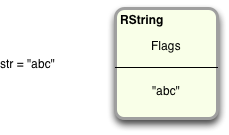
\includegraphics[width=0.29\textwidth]{images/gc/gc01-rstring.png}
	\caption{Representación gráfica de la estructura \textit{RString}.}
\end{figure}
\bigskip

\noindent En la parte inferior tenemos los datos de la cadena en sí, mientras que en la parte superior hemos puesto la palabra \textit{Flags} (banderas) para representar diferentes valores de los metadatos internos acerca de la cadena que es rastreada por Ruby. Resulta que todos los valores utilizados por el programa hecho en Ruby se guardan en estructuras similares a \textit{RString} denominadas \textit{RArray}, \textit{RHash}, \textit{FICH\_R}, etc. Todos ellos comparten el mismo diseño básico: algunos datos y el mismo conjunto de flags. El nombre común para este tipo de estructura, que se comparte entre todos los tipos de objetos internos, es \textit{RValue}, lo que significa ``Ruby Value'' (Valor de Ruby).
	\par
	Ruby asigna y organiza estas estructuras \textit{RValue} en conjuntos llamados \textit{heaps}. En la \textit{Figura 2} se muestra un diagrama conceptual del arreglo heap de Ruby, el cual contiene los tres valores de la cadena junto con algunos otros \textit{RValue's}.
\bigskip

\begin{figure}[h]
	\centering
	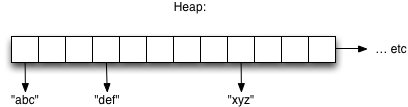
\includegraphics[width=0.55\textwidth]{images/gc/gc02-heap.png}
	\caption{Diagrama conceptual del arreglo heap de Ruby.}
\end{figure}
\bigskip

	A medida que una aplicación hecha en Ruby se ejecuta, siempre que se crea una nueva variable o el valor de algún tipo, el intérprete de Ruby encuentra una estructura \textit{RValue} disponible en el heap y la usa para almacentar el nuevo valor. Por supuesto, todo esto es manejado de forma automática, sin dar problemas a quien se encuentra programando.
	\par
	Pero el lector se preguntará: \textit{¿Qué ocurre cuando las estructuras RValue en el heap se acaban, cuando no quedan mas para almacenar nuevos valores requeridos por la aplicación?} En realidad, esto ocurre con mas frecuencia de lo que cabría esperar debido a que hay muchas estructuras \textit{RValue} creadas internamente por Ruby de las cuales no somos conscientes. De hecho, el mismo código del programa es convertido en un gran número de estructuras \textit{RValue}, es parseado y por último, convertido en byte code.
	\par
	Cuando no hay mas estructuras \textit{RValue} disponibles y el programa necesita almacenar un valor nuevo, Ruby ejecuta el código del \textit{recolector de basura (GC)}. El trabajo del recolector de basura es encontrar cual de los \textit{RValues} ya no se encuentran referenciados por la aplicación, pudiendo ser reciclado y reutilizado por otro valor. Veámos como funciona a un alto nivel.
	\par
	Primeramente, el código del GC ``marca'' todas las estructuras \textit{RValue} activas. Es decir, recorre todas las variables y otras referencias activas que posee el programa como estructuras \textit{RValue}, y marca cada una usando uno de los indicadores internos de flag denominado \textit{FL\_MARK} (\textit{Figura 3}).
\bigskip

\begin{figure}[h]
	\centering
	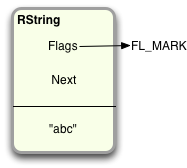
\includegraphics[width=0.25\textwidth]{images/gc/gc03-fl-mark.png}
	\caption{Marcado de un RValue con el indicador FL\_MARK.}
\end{figure}
\bigskip
	
	Lo hasta aquí expuesto es solo la mitad de lo que realiza el algoritmo del recolector de basura por marcado y barrido de Ruby. Algo a tener en cuenta es que las estructuras marcadas son usadas activamente por el programa y no pueden ser liberadas o reutilizadas.
	\par
	Una vez que todas las estructuras en el sistema están marcadas, las estructuras restantes son barridas hacia una lista simplemente enlazada usando el puntero \textit{Next} de cada estructura \textit{RValue}. En el diagrama de la \textit{Figura 4} se representa el flag de \textit{FL\_MARK} en el arreglo heap con la letra ``M'', y por debajo se puede muestra la lista de los \textit{RValue} sin marcar, denominada la \textit{lista libre}. 

\begin{figure}[h]
	\centering
	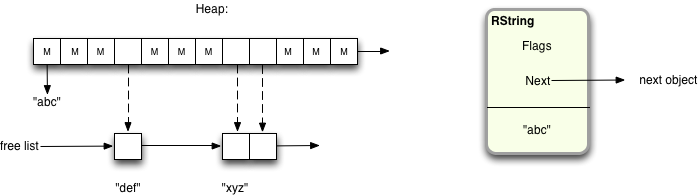
\includegraphics[width=1\textwidth]{images/gc/gc04-free-list.png}
	\caption{Marcado de un RValue con el indicador FL\_MARK.}
\end{figure}
	
	Como se ha de imaginar el lector, la lista libre puede ahora ser usada para proveer nuevas estructuras \textit{RValue} al programa, ya que este último nunca se detiene. Ahora, cada vez que el programa hecho en Ruby asigna un nuevo objeto o valor, este usa una estructura \textit{RValue} de la lista libre al mismo tiempo que es removida de dicha lista. Eventualmente, la lista libre se comenzará a vaciar nuevamente y Ruby deberá ejecutar nuevamente el recolector de basura.
	\par
	Después de un tiempo puede que no queden estructuras sin marcar en el heap, es decir, todas las \textit{RValues} disponibles puede que estén siendo utilizadas activamente. En esos casos, Ruby asignará un heap nuevo con mas estructuras \textit{RValue}. En realidad, asigna nuevos heaps de diez a la vez. Una aplicación típica de Ruby podría llegar a tener muchos arreglos heap diferentes.
\bigskip


%% RECOLECCIÓN DE BASURA - El porvenir de Ruby 2.0: Bitmap Marking GC
\subsection{El porvenir de Ruby 2.0: \textit{Bitmap Marking GC}}

	Ruby es un lenguaje en constante progreso. Tal es así que para la nueva futura versión de esta, \textit{Ruby 2.0}, se ha dado a conocer un cambio muy significativo: un nuevo algoritmo para el recolector de basura llamado \textit{Bitmap Marking}. El desarrollador detrás de este sofisticado e innovador cambio es nuevamente Narigiro Nakamura, quien ha estado trabajando en este desde el 2008.
	\par
	El nuevo algoritmo \textit{Bitmap Marking GC} promete reducir drásticamente el consumo total de memoria de los procesos de Ruby que se ejecutan en un servidor web. Prácticamente hablando, esta nueva implementacion del GC ayudará al MRI de Ruby 2.0 a trabajar mas eficientemente en entornos de producción de servidores web reduciendo el consumo de memoria. 
	\par
	El propósito de este apartado es unicamente informativo, por lo que no profundizaremos sobre como es el funcionamiento del nuevo algoritmo\footnote{''Para más información acerca de cómo es que trabaja el ``Bitmap Marking GC'' diríjase a http://patshaughnessy.net/2012/3/23/why-you-should-be-excited-about-garbage-collection-in-ruby-2-0}. 


%EL INTERPRETE DE RUBY
\section{El interprete de Ruby}

Como lo enunciamos en el comienzo del informe, Ruby es un lenguaje de scripts interpretado para una programación orientada a objetos rápida y sencilla. En esos principios (ver sección 4) son en los que se centro Matz en su rol de diseñador de lenguaje de programación Ruby. Matz implemento el primer interprete de ruby sin preocuparse demasiado por los problemas de performance y priorizando los principios de diseño de lenguaje de Ruby. A medida que el lenguaje se fue populrizando se tomo más en serio el problema de performance general debido al interprete.

\subsection{MRI: El primer interprete}

La crítica más habitual de Ruby es el pobre rendimiento del intérprete frente a otros lenguajes rivales. Las cifras indican que por lo general para un mismo algoritmo el intérprete de Ruby ofrece un menor rendimiento que Python, PHP, Perl ... pudiendo poner en la lista cualquiera de los lenguajes más populares.

 El intérprete de Ruby escrito por Matz, conocido como MRI (de Matz Reference Implementation, o Implementación de Referencia de Matz) adolece de no pocos problemas (hay quien afirma que un lenguaje como C no es buena elección a la hora de implementar lenguajes dinámicos)

En todo caso, la comunidad de Rubistas (con Matz a la cabeza) hace tiempo que ha asumido el problema de rendimiento en la MRI y han surgido no pocos proyectos para corregir esta deficiencia. Uno de los problemas con los que se enfrentan los valientes que desean implementar un lenguaje es que el lenguaje Ruby no dispone de una especificación funcional. Por tanto, la única fuente fiable de documentación sobre los entresijos del lenguaje Ruby es el estudio del código fuente en C del intérprete escrito por Matz (de ahí el nombre MRI)


\subsection{YARV (o KRI)}

YARV (yeat another ruby interprete) de Sasada Koich es  la reimplementación de Ruby usando su propia máquina virtual y un compilador a código de bytes. El trabajo de Sasada Koichi, basado en un enfoque más moderno que la implementación de Matz, es tan brillante que forma parte de las versiones oficiales 1.9.x de Ruby. Aún hay algún trabajo por hacer con el problema de performance de Ruby pero cabe destacar que, por lo general, una aplicación Rails verá mejoras de rendimiento del 15% sólo por usar YARV.

YARV divide el problema de la implementación del lenguaje en dos etapas: un compilador de código de bytes y una máquina virtual que ejecuta dicho bytecode. Surge de manera natural la pregunta de si no sería posible usar alguna máquina virtual ya existente y generar bytecode compatible con ella. Si hablamos de máquinas virtuales, la de Java está más que probada.

\subsection{Otros interpretes para ruby}

JRuby consiste en escribir un intérprete Ruby escrito en Java. Una de las ventajas de ejecutar Ruby en una máquina virtual de Java, por supuesto, es tener acceso a código ya existente escrito en Java lo cual hace a JRuby la implementación ideal para integrar Rails en entornos enterprise. Otra ventaja es que JRuby por definición se verá beneficiado de las mejoras posteriores que se realicen en el intérprete Java. JRuby es un intérprete de Ruby escrito en Java, XRuby es un traductor de Ruby a bytecode de Java (o lo que es lo mismo, de un fichero .rb generará un .class) Este traductor está basado en ANTLR. XRuby ya es capaz de generar bytecode Java para toda la librería estándar de Ruby y para Ruby on Rails 1.2.x

Rubinius es otro interprete cuyo enfoque consiste en escribir la mayor parte del lenguaje en Ruby y dejar que la máquina virtual -escrita en C- ejecute el menor subconjunto posible de funcionalidad. En concreto, Rubinius pone el énfasis en el recolector de memoria y la implementación de forks y threads. A destacar que Rubinius parece surgir del mundo Rails (Evan Phoenix trabaja en Engine Yard, proveedores de alojamiento avanzado Rails) por tanto buena parte de las mejoras que promete en el intérprete atacan a los problemas de rendimiento que más pueden aquejar a nuestras aplicaciones Rails.


% RUBY ON RAILS: UN PUNTO FUERTE DEL LENGUAJE
\section{\textit{Ruby On Rails}: un punto fuerte del lenguaje}

	En la actualidad, Ruby se ha popularizado en el mundo del desarrollo de las aplicaciones webs a través del framework \textit{Ruby On Rails}, o mas comúnmente conocido como \textit{Rails}, escrito en este mismo lenguaje.
	\par
	Ruby on Rails nace como un framework de desarrollo web especialmente diseñado con un fin en particular: hacer la vida más fácil a las personas que desarrollan aplicaciones destinadas a la web. Muchas de estas personas quiza se sientan frustradas con tecnologias como PHP, Java o .NET, que si bien son buenas, conllevan problemas de carga de recursos y una complejidad innecesaria. Ruby on Rails es simplemente más sencillo.
	\par
	Rails utiliza el patrón MVC para poder administrar sus recursos. Si bien Java utiliza distintos frameworks también basados en MVC, Rails lleva el concepto mucho mas allá debido a que hay un lugar específico para cada parte del codigo, y cada componente de nuestra aplicación funciona de manera estándar. Es decir, es como si iniciaramos una aplicacion con el esqueleto previamente armado.
	\par
	Todas estas potenciales caracteristicas hicieron que Ruby on Rails sea una de las razones por las que el lenguaje de programación Ruby ha logrado un importante impulso, siendo cada vez mas reconocido como una buena opción a la hora de elegir un lenguaje con el que llevar a cabo un proyecto.




% APLICACIONES
\section{Aplicaciones}

Con el paso del tiempo Ruby fue siendo utilizado por un número cada vez mayor de desarrolladores para llevar a cabo proyectos de grande envergadura. A continuación se muestra un listado de aplicaciones\footnote{''Véase una lista mas completa de aplicaciones en los siguientes vínculos: http://rubyonrails.org/applications\\http://www.ruby-lang.org/en/documentation/success-stories''} realizadas en este lenguaje:
\bigskip\\

\textbf{Web:}
\begin{itemize}
	\itemsep=1pt \topsep=0pt \partopsep=0pt \parskip=0pt \parsep=0pt
	\item Twitter (\textit{http://www.twitter.com})
	\item Shopify (\textit{http://www.shopify.com})
	\item Groupon (\textit{http://www.groupon.com})
	\item XING (\textit{http://www.xing.com})
\end{itemize}
\medskip

\textbf{Simulaciones:}
\begin{itemize}
	\itemsep=1pt \topsep=0pt \partopsep=0pt \parskip=0pt \parsep=0pt
	\item NASA Langley Research Center: usa Ruby para llevar a cabo simulaciones. (\textit{http://www.larc.nasa.gov})
	\item Motorola (\textit{http://www.motorola.com})
\end{itemize}
\medskip

\textbf{Modelado 3D:}
\begin{itemize}
	\itemsep=1pt \topsep=0pt \partopsep=0pt \parskip=0pt \parsep=0pt
	\item Google SketchUp: SketchUp incluye una interfaz de programación de aplicaciones (API) para usuarios familiarizados con Ruby que deseen ampliar las funciones de SketchUp. Esta interfaz permite crear herramientas, opciones de menú y otros complementos, como generadores automáticos de componentes, que se incluirán en los menús de SketchUp. (\textit{http://sketchup.google.com})
\end{itemize}
\medskip

\textbf{Telecomunicaciones:}
\begin{itemize}
	\itemsep=1pt \topsep=0pt \partopsep=0pt \parskip=0pt \parsep=0pt
	\item Open Domain Server (ODS): permitir a los usuarios el uso de DNS dinámicos. (\textit{http://ods.org})
	\item Lucent: uso en producto de telefonía wireless 3G. (\textit{http://www.lucent.com})
\end{itemize}
\medskip




% UN EJEMPLO PRACTICO DE APLICACIÓN
\section{Un ejemplo práctico de aplicacion}





% CONCLUSIÓN
\section{Conclusión}




\end{document}
